\documentclass[t]{beamer}

\usetheme{CambridgeUS}
\usecolortheme{beaver}
\setbeamertemplate{navigation symbols}{}

\usepackage[utf8]{inputenc}
\usepackage[croatian]{babel}

\usepackage{datetime}
\renewcommand{\dateseparator}{.}
\newcommand{\todayiso}{\twodigit\day \dateseparator \twodigit\month \dateseparator \the \year}
\date{\todayiso}

\usepackage{listing}
\usepackage{graphicx}
\usepackage{subcaption}
\captionsetup{compatibility=false}

\title[NKOSL]{Napredno korištenje operacijskog sustava Linux}
\author[Dominik Barbarić]{Dominik Barbarić\\{\small Nositelj: doc.dr.sc. Stjepan Groš}}
\subtitle{8. Virtualizacija}
\institute[FER]{Sveučilište u Zagrebu\\Fakultet elektrotehnike i računarstva}

\begin{document}
	
	{
		\setbeamertemplate{footline}{}
		\begin{frame}
			\maketitle
		\end{frame}
	}
	
	\begin{frame}
		\frametitle{Sadržaj}
		\tableofcontents
	\end{frame}


\section{Virtualizacija}


\begin{frame}
	\frametitle{Virtualizacija}

	\begin{itemize}
		\item Emulacija fizičkog računala na hostu
		\item Bolja iskorištenost resursa
		\item Jednostavnije upravljanje
	\end{itemize}
	
	\begin{itemize}
		\item Virtualizacija dijeli resurse fizičkog računala na više emuliranih računala
		\item Virtualna računala i fizičko računalo su međusobno izolirani
	\end{itemize}
\end{frame}


\begin{frame}
	\frametitle{Virtualizacija}
	\begin{columns}[T]
		\begin{column}{0.5\textwidth}
			\centering
			Bez virtualizacije\\
			\vspace{1em}
			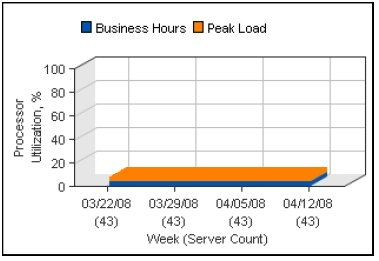
\includegraphics[width=0.9\textwidth]{no_virt_chart.jpg}
			\vspace{1em}
			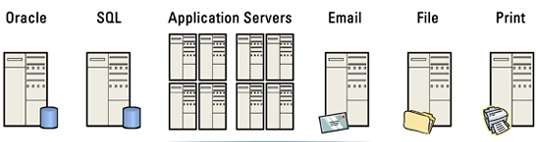
\includegraphics[width=0.8\textwidth]{no_virt_apps.jpg}
		\end{column}
		\begin{column}{0.5\textwidth}
			\centering
			Virtualizacija\\
			\vspace{2em}
			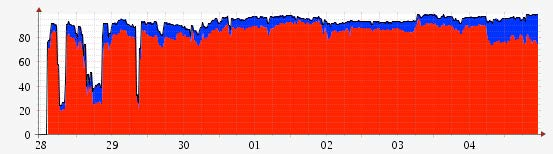
\includegraphics[width=\textwidth]{virt_chart.jpg}
			\vspace{1em}
			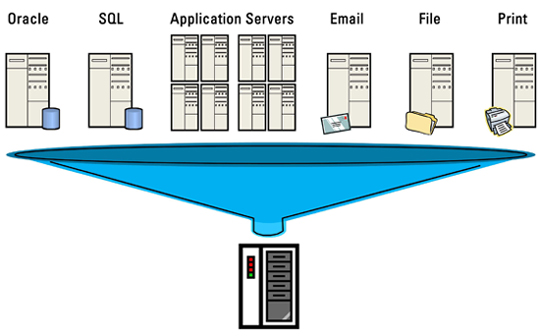
\includegraphics[width=0.9\textwidth]{virt_apps.jpg}
		\end{column}
	\end{columns}
\end{frame}




\section{Tehnike virtualizacije}

\begin{frame}
	\frametitle{Guest OS virtualizacija}
	\centering
	\begin{itemize}
		\item Virtualizaciju obavlja aplikacija unutar koje se pokreće cijeli operacijski sustav virtualnog računala
	\end{itemize}
	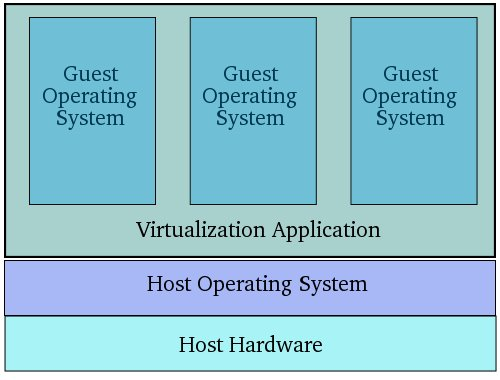
\includegraphics[width=0.65\textwidth]{guest_virt.jpg}
\end{frame}

\begin{frame}
	\frametitle{Shared kernel virtualizacija}
	\centering
	\begin{itemize}
		\item Virtualna računala dijele zajednički (Linux / UNIX) kernel
	\end{itemize}
	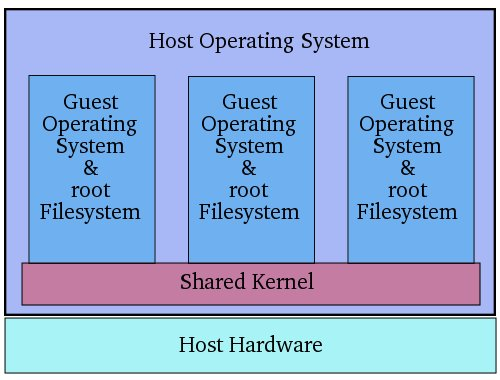
\includegraphics[width=0.65\textwidth]{shared_virt.jpg}
\end{frame}

\begin{frame}
	\frametitle{Kernel virtualizacija}
	\centering
	\begin{itemize}
		\item Kernel ima podršku za virtualizaciju
	\end{itemize}
	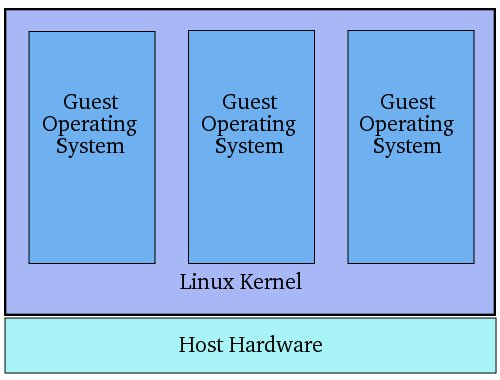
\includegraphics[width=0.65\textwidth]{kernel_virt.jpg}
\end{frame}

\begin{frame}
	\framesubtitle{Hypervisor}
	\centering
	\begin{itemize}
		\item Operacijski sustav namijenjen virtualizaciji
	\end{itemize}
	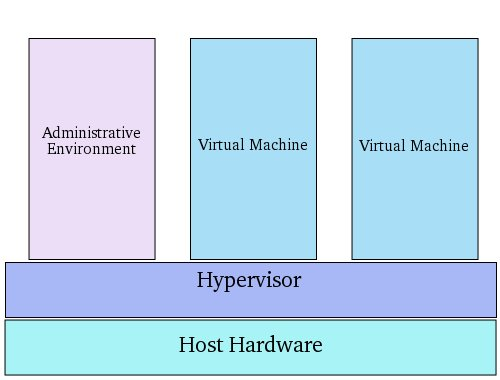
\includegraphics[width=0.65\textwidth]{hypervisor_virt.jpg}
\end{frame}


\section{cgroups}

\begin{frame}
	\frametitle{cgroups}
	\begin{itemize}
		\item Control groups
	\end{itemize}
	\begin{itemize}
		\item Grupiranje procesa i razdjela resursa
		\begin{itemize}
			\item Limitiranje resursa
			\item Prioriteti grupa procesa
			\item Pokretanje i zaustavljanje grupa procesa
		\end{itemize}
		\item \emph{Namespace isolation}
		\begin{itemize}
			\item \emph{Skrivanje} resursa koji nisu dodijeljeni procesu
		\end{itemize}
	\end{itemize}
\end{frame}

\begin{frame}[fragile]
	\frametitle{cgroups}
	\scriptsize
	\begin{verbatim}
# cgcreate -a user -g memory,cpu:groupname
$ ls -l /sys/fs/cgroup/memory/groupname
total 0
-rwxrwxr-x 1 user root 0 Sep 25 00:39 cgroup.event_control
-rwxrwxr-x 1 user root 0 Sep 25 00:39 cgroup.procs
-rwxrwxr-x 1 user root 0 Sep 25 00:39 cpu.rt_period_us
-rwxrwxr-x 1 user root 0 Sep 25 00:39 cpu.rt_runtime_us
-rwxrwxr-x 1 user root 0 Sep 25 00:39 cpu.shares
-rwxrwxr-x 1 user root 0 Sep 25 00:39 notify_on_release
-rwxrwxr-x 1 user root 0 Sep 25 00:39 tasks
$ cgexec   -g memory,cpu:groupname/foo bash
	\end{verbatim}

\end{frame}



\section{lxc}

\begin{frame}[fragile]
	\frametitle{LXC}

	\begin{itemize}
		\item Linux containers
		
		\item Shared kernel virtualizacija
		\item Implementira cgroups
	\end{itemize}

	\begin{itemize}
		\item Virtualna računala se kreiraju pomoću template skripti \texttt{/usr/share/lxc/templates}
		\item Defaultno instalacija u \texttt{/var/lib/lxc/NazivVM}
	\end{itemize}
	
	\scriptsize
	\begin{verbatim}
# lxc-create -n archVM -t /usr/share/lxc/templates/lxc-archlinux
# lxc-start -n archVM
# lxc-attach -n archVM
# lxc-stop -n archVM
	\end{verbatim}

\end{frame}


\begin{frame}
	\frametitle{KVM}
	\begin{columns}[T]
	\begin{column}{0.5\textwidth}
		\begin{itemize}
			\item Kernel-based Virtual Machine
			\item Hypervisor
			\item U Linux kernelu od 2007.
		\end{itemize}
	\end{column}
	\begin{column}{0.5\textwidth}
		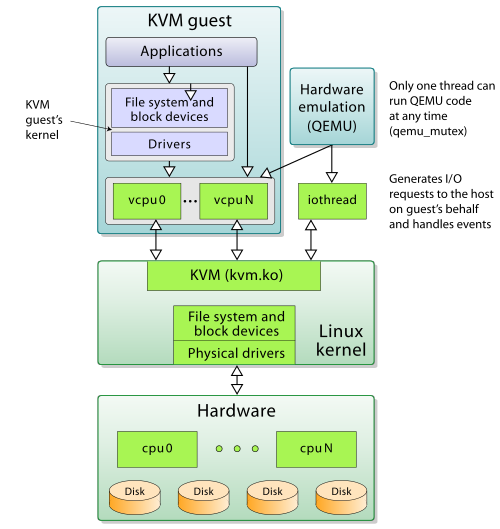
\includegraphics[width=\textwidth]{kvm.png}
	\end{column}
	\end{columns}
\end{frame}


\begin{frame}[fragile]
	\frametitle{QEMU}
	\begin{itemize}
		\item Quick Emulator
	\end{itemize}
	\begin{itemize}
		\item Emulira različite arhitekture neovisno o arhitekturi hosta
		\item Userspace virtualizator za KVM i Xen
	\end{itemize}
	\vfill
	\small
	\begin{verbatim}
$ qemu-img create -f raw disk.img 4G
$ qemu-system-i386 -cdrom fedora.iso -boot order=d disk.img
	\end{verbatim}
\end{frame}


\begin{frame}
	\frametitle{Literatura}
	\url{http://www.virtuatopia.com/index.php/An_Overview_of_Virtualization_Techniques}
	\vfill
	\url{https://wiki.archlinux.org/index.php/Cgroups}\\
	\url{https://www.kernel.org/doc/Documentation/cgroups/cgroups.txt}
	\vfill
	\url{https://wiki.archlinux.org/index.php/Linux_Containers}
	\vfill
	\url{https://wiki.archlinux.org/index.php/QEMU}
	\vfill
	\url{http://www.linux-kvm.org/page/Main_Page}
\end{frame}


\end{document}